%Qué resultados obtuvimos del análisis en cuestión. Acá vamos a poner qué palabras fueron significativas, dónde lo fueron, y demás.

% Distribucion de entropía vs frecuencia  
% Distribucion de frecuencias de las palabras
% Distr entropia
% de valor de la inf. a partir de los 5000 se ve que se estanca (graficar hasta 10**5)

% subsection de la region de las palabras --> muestro tabla
% se muestra que las regiones son contiguas geograficamente (hablarlo con santiago)

% Las palabras que se vieron, las primeras generalmente se refieren a lugares o gentilicios



% ver los graficos que hace zanette en su paper

% se busco el dataset de localidades para filtrar las palabras que son lugares

\section{Entropía}
Teniendo el listado de palabras hicimos un cálculo de entropía tomando en cada provincia la cantidad de ocurrencias de cada palabra. En la figura \ref{fig:entropiaPalabras} podemos observar la distribución del valor de la entropía sobre todas las palabras con más de 40 ocurrencias y dichas por más de 5 usuarios.

Podemos ver que la mayor parte de las palabras tienen un valor de entropía entre 2.5 y 3. Esto quiere decir que hay un gran conjunto de palabras que tiene una cantidad de ocurrencias relativamente uniforme a lo largo de todas las provincias. Sin embargo hay otro conjunto de palabras que tienen una entropía menor a 2, la cual podemos considerar como baja. Estas últimas palabras serán las que tienen mayor interés debido a que tienen una variación marcada en cuanto a su utilización en las distintas regiones.

Sin embargo, ver solamente la entropía de las palabras nos puede generar la detección de palabras que no son de interés, ya sea porque no ocurren una cantidad significativa de veces o porque la variación de las ocurrencias en las distintas provincias se debe solamente a pocos usuarios que la utilizan mucho. Es por esto que también se calculó la entropía teniendo como variable la cantidad de personas que utilizaron cierto término en una determinada provincia.


\begin{figure}[ht]
\centering
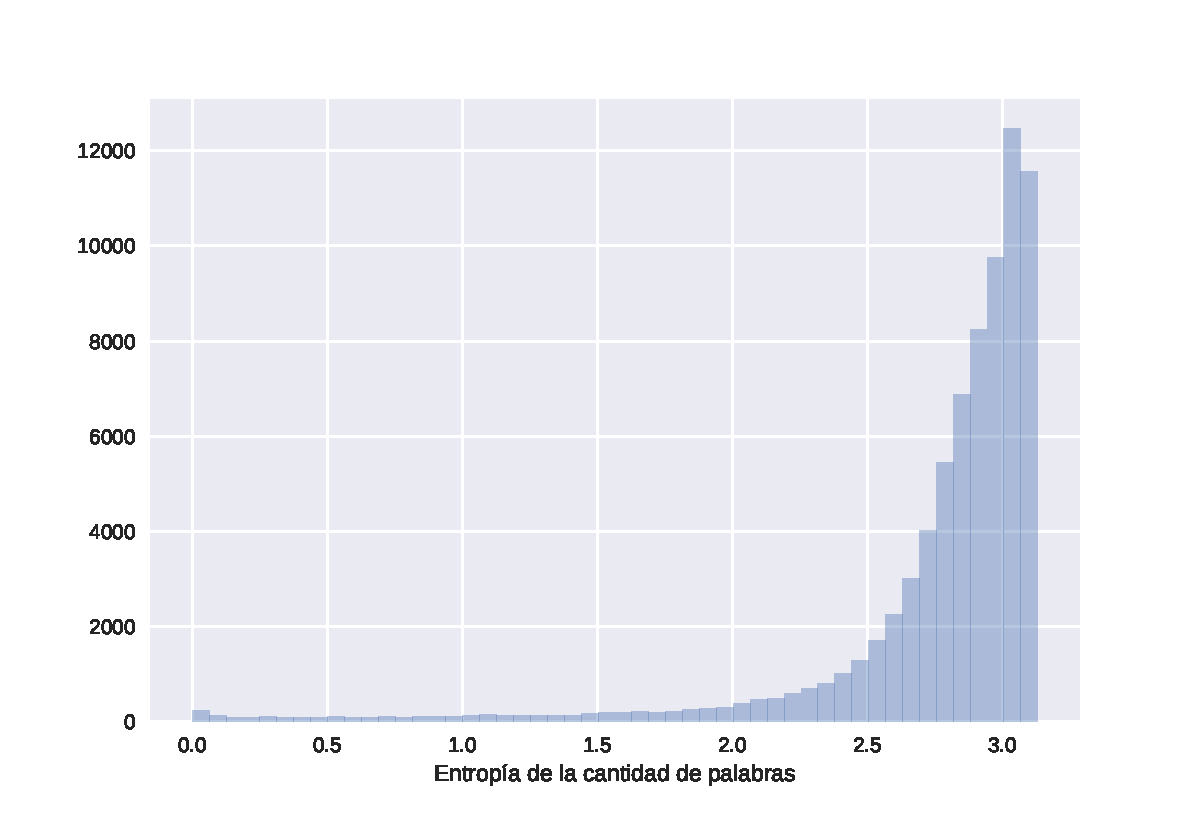
\includegraphics[width=1.0\textwidth]{./images/DistribucionEntropia.pdf}
\caption{Histograma del valor de la entropía de las palabras ($H_w$).} 
\label{fig:entropiaPalabras} 
\end{figure}



\section{Valor de la información}
\label{sec:ValorDeLaInformacion}
En el gráfico \ref{fig:infoValue} se muestra una clara relación entre la cantidad de ocurrencias que tiene una palabra y su valor de la información, indicado por el colo: cuanto más oscuro más alto el valor. A su vez, se nota que el valor de la información suele ser mayor a medida que el valor de la entropía es menor. Esto no siempre es el caso debido a que hay palabras que tiene una entropía de palabras baja, pero sin embargo la entropía de personas es alta logrando que el valor de la información sea bajo.

\begin{figure}[ht]
\centering
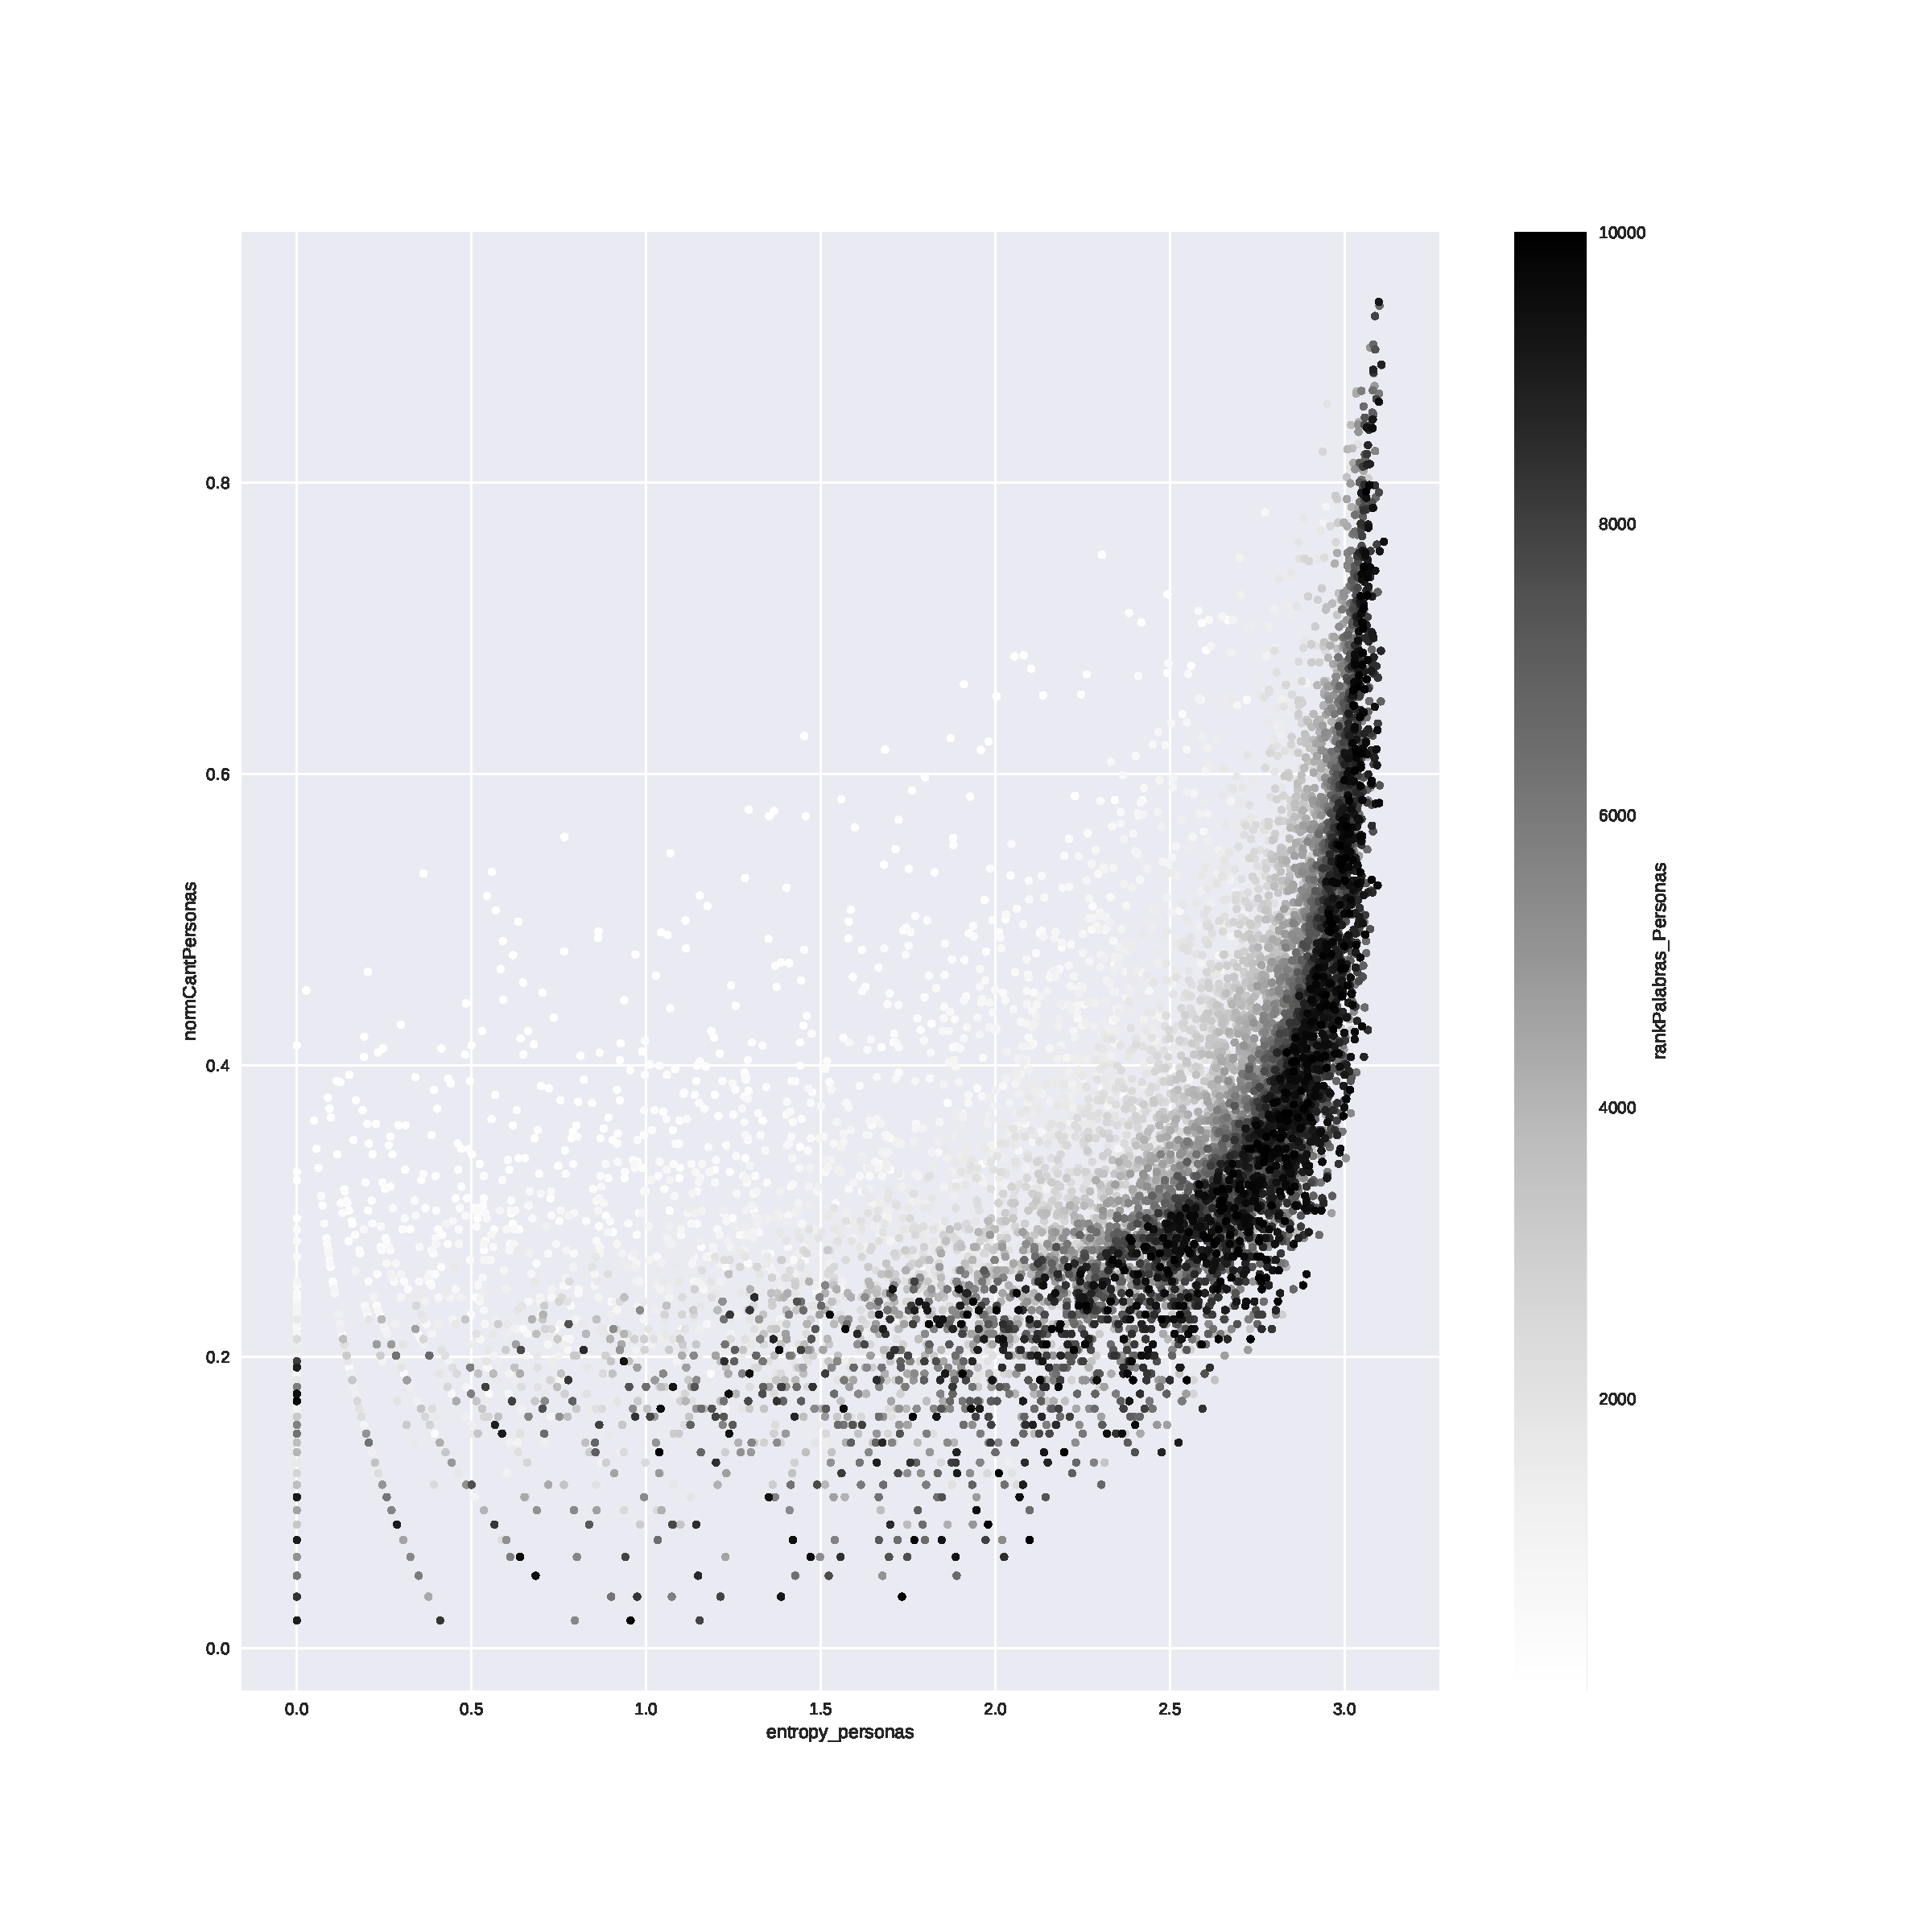
\includegraphics[width=1.0\textwidth]{./images/entropiaPersonasxNormCantPersonas.pdf}
\caption{Gráfico de dispersión que muestra la posición en el listado ordenado según el valor de la información a partir de la escala cromática. Las posiciones más bajas aparecen más blancas. A su vez se muestra para cada palabra el valor de la entropía de las personas ($H_u$) y la cantidad normalizada de personas que utiliza dicho término($norm_p$). } 
\label{fig:infoValue} 
\end{figure}

En la figura \ref{fig:ivalue} se puede ver el valor de la información según la posición en la que se encuentra en el listado ordenado por la métrica. Notamos que el valor se estabiliza aproximadamente a partir de la palabra cuya posición es 4000 acercándose a 0.


\begin{figure}[ht]
\centering
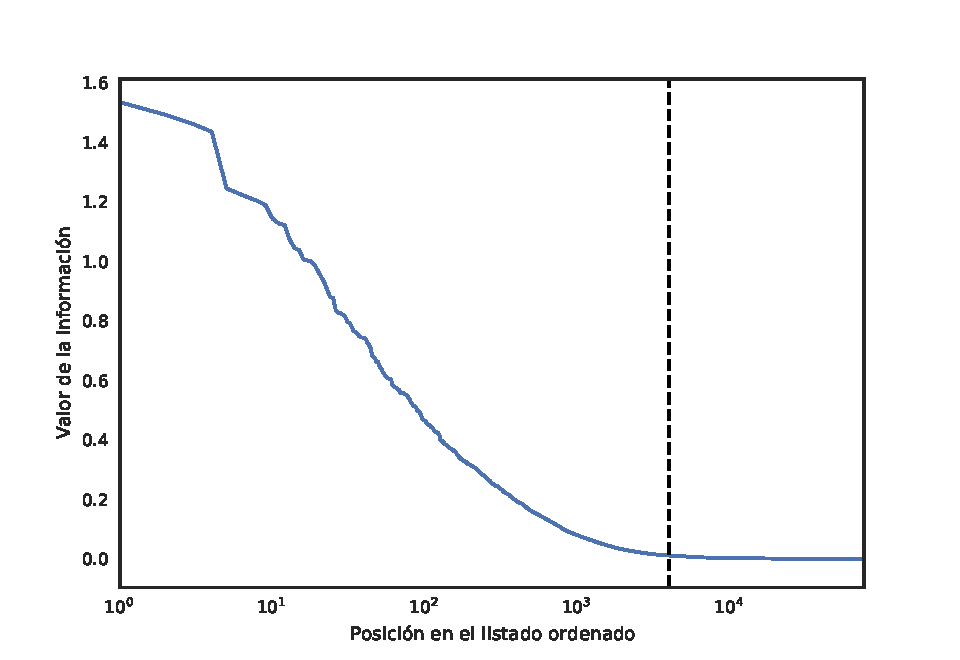
\includegraphics[width=0.6\textwidth]{./images/train/conFiltro/valorInformacionCorte.pdf}
\caption{Distribución del valor de la información según la posición de la palabra en el listado de palabras. El gráfico se realizó sobre el conjunto de palabras cuya cantidad de ocurrencias era mayor a 40 y la cantidad de usuarios que utilizaron cada término era mayor a 5. } 
\label{fig:ivalue}
\end{figure}


\section{Proporción acumulada de ocurrencias} % (fold)
\label{proporcionDeOcurrencias}

Para tener una mejor noción sobre la métrica, medimos el porcentaje de las ocurrencias de las palabras que muestran contrastes según nuestra métrica cubiertas por subconjuntos de provincias de manera tal que para cada palabra y un número fijo de provincias, la región con esa cantidad de provincias tenga un cubrimiento máximo. 
En la figura \ref{fig:propAcum} mostramos la proporción acumulada de las palabras, tomando diferentes muestras de palabras. Es notable la diferencia de proporciones acumuladas según la muestra de palabras. Solamente con una provincia para cada palabra ya se puede cubrir, en promedio, el 76\% del total de ocurrencias sobre las mil palabras con mayor valor de la información.

En el gráfico \ref{fig:propAcum5000} se observa que la variación del cubrimiento de ocurrencias es menor a medida que se aumenta la cantidad de provincias. 



\begin{figure}[!ht]\centering
  \begin{minipage}{0.49\textwidth}
    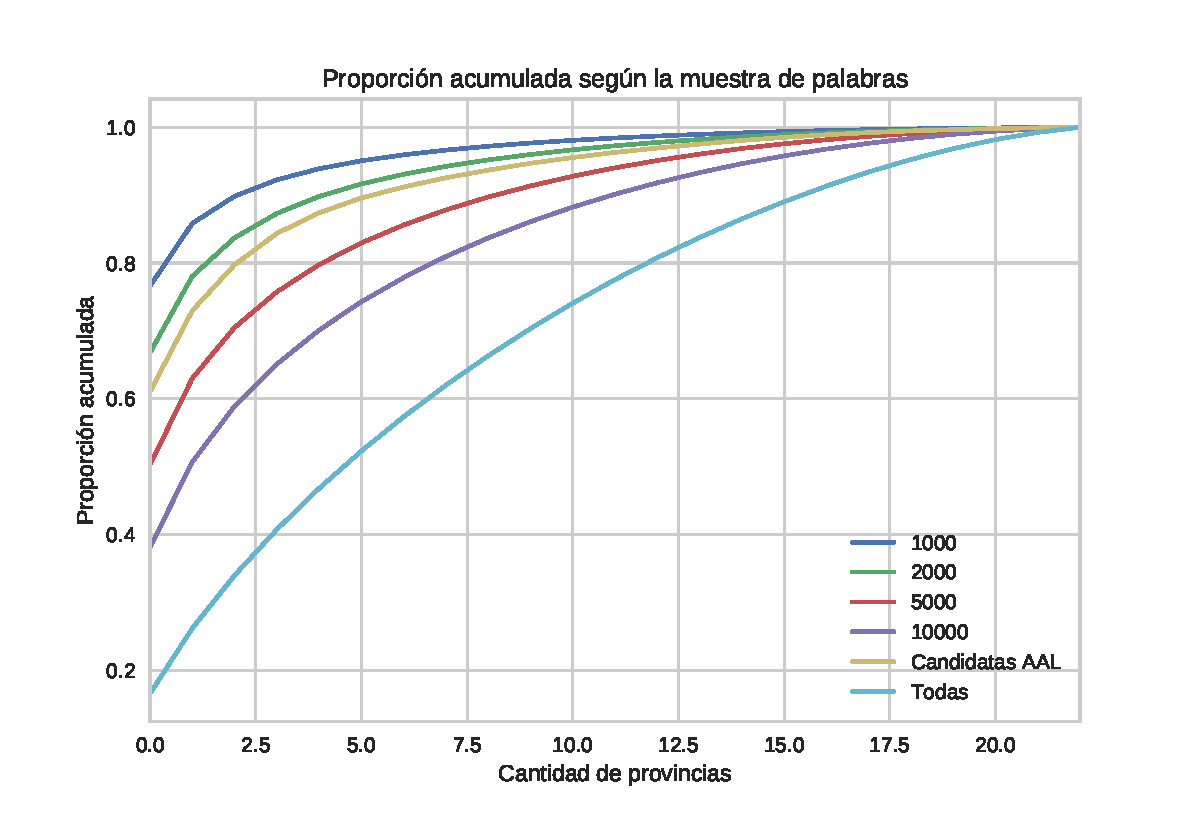
\includegraphics[width=\linewidth]{./images/PropAcum.pdf}
    \caption{Proporción de ocurrencias acumulada según la muestra de palabras.} 
    \label{fig:propAcum} 
   \end{minipage}
   \begin{minipage}{0.49\textwidth}
    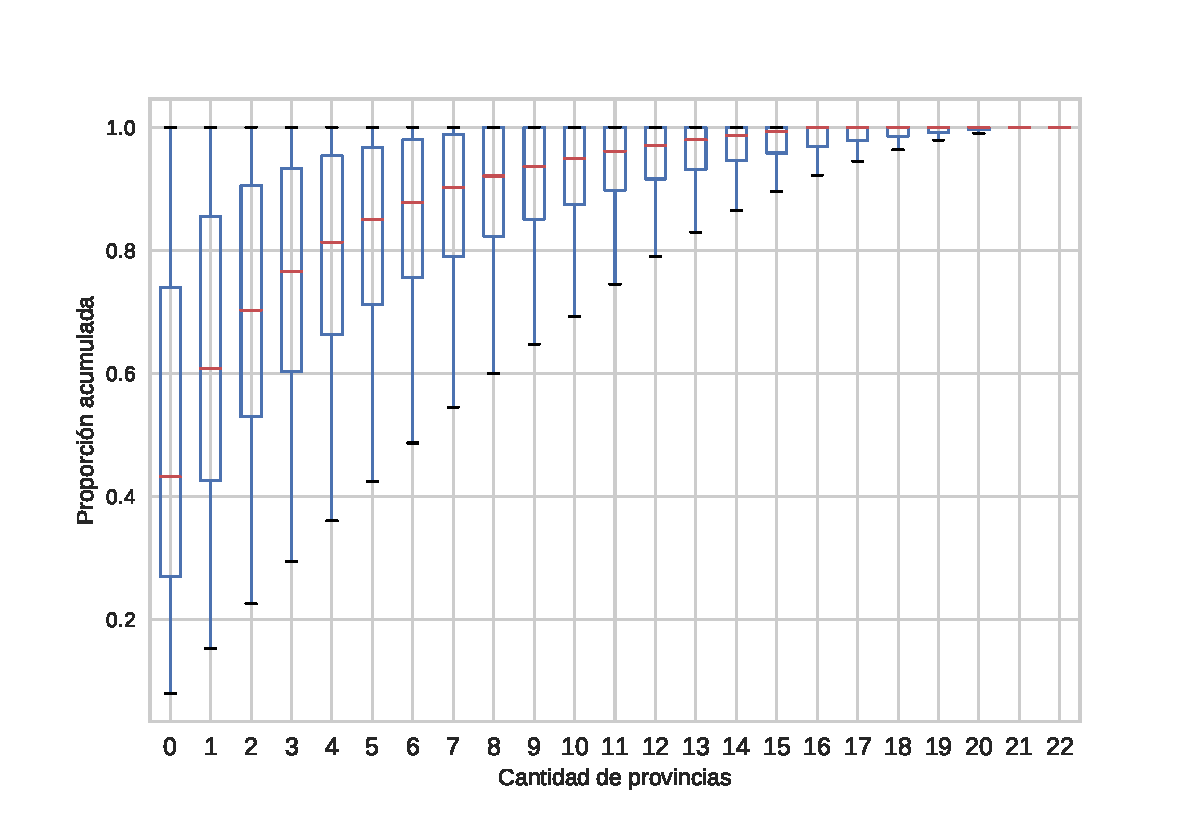
\includegraphics[width=\linewidth]{./images/PropAcum5000.pdf}
    \caption{Variación de la proporción de ocurrencias acumulada a partir de la muestra con las primeras 5000 palabras con mayor valor de la información.} 
    \label{fig:propAcum5000} 
   \end{minipage}
   
\end{figure}

% \begin{figure}[h]
% \centering
% 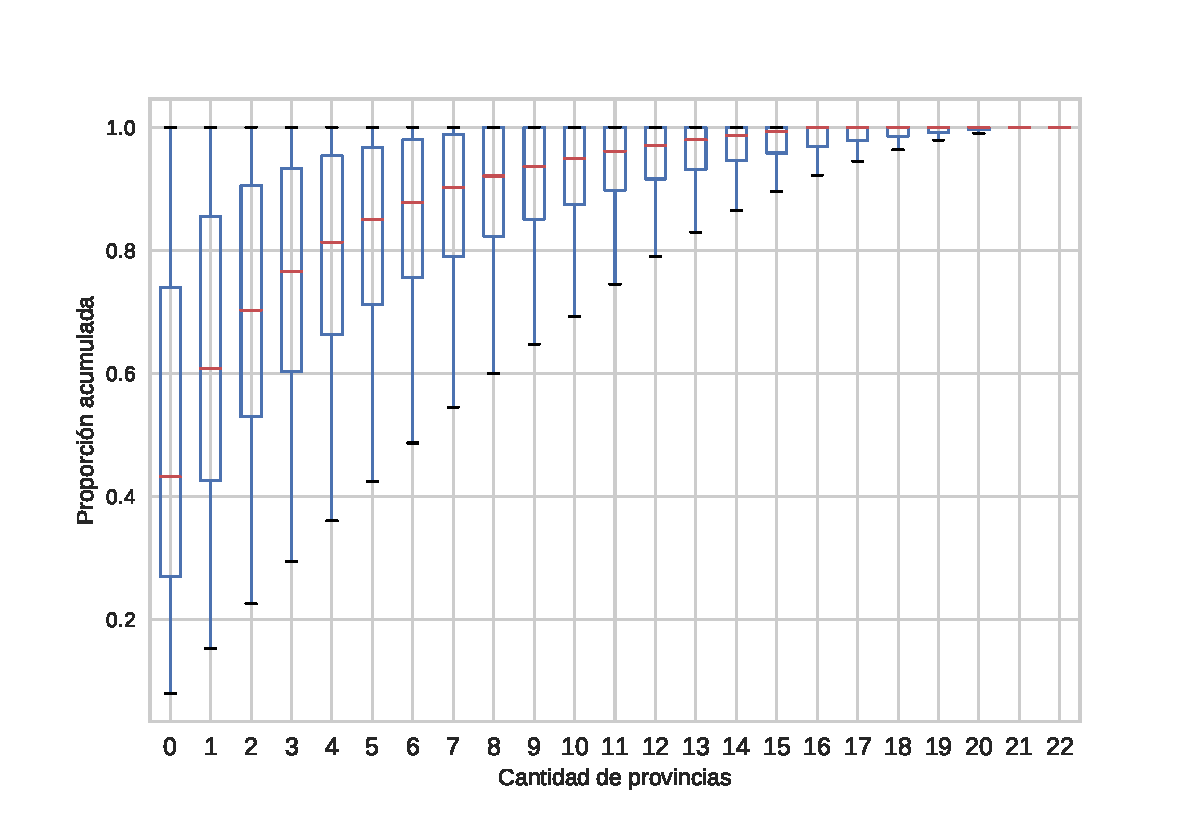
\includegraphics[width=0.5\textwidth]{./images/PropAcum5000.pdf}
% \caption{Proporciones Acumuladas} 
% \label{fig:propAcum5000} 
% \end{figure}

\section{Palabras candidatas} % (fold)
\label{palabras_candidatas}
Para buscar las palabras candidatas a tener contrastes significativos en cuanto a la cantidad de ocurrencias en distintas provincias, elegimos el conjunto de las primeras 
cinco mil (5000) palabras con valor de la información más altas. El número 5000 surgió de ver la distribución de los valores de la información. Cómo se puede ver en 
el gráfico \ref{fig:ivalue} hay una caída pronunciada de la métrica y a partir de la palabra cuya posición es 4000 se ve que empieza a estabilizarse y los valores son 
muy cercanos a 0. Es por esto que nos pareció razonable dar un margen de 5000 palabras para evaluar manualmente las palabras del listado y entre estas seleccionar las palabras con contrastes significativos que tienen interés a nivel lingüístico.

Como era de esperar las ciudades y provincias son palabras que ocurren mayormente en sus respectivas regiones. Es por esto que tienen una gran variación en 
la cantidad de ocurrencias en las distintas provincias, lo que genera un valor alto en la métrica de valor de la información. Para detectar las palabras que tienen 
mayor interés lingüístico buscamos un conjunto de datos con los nombres de las localidades y departamentos de la República Argentina de modo tal que podamos resaltar para que el equipo de filólogos tenga una primera alerta sobre posible toponimia.

% Agregar algún comentario sobre regiones dialectales conocidas


\subsection{Regiones de palabras} % (fold)
\label{sub:regiones_de_palabras}

Una vez que calculamos las regiones que cubren un umbral para cada palabra, nos propusimos analizar cuales son las más frecuentes. Para eso generamos una lista con los conjuntos de provincias cuya cantidad sea menor o igual a 6 y los ordenamos según su frecuencia. En la tabla \ref{tab:regiones} se muestran los primeros conjuntos de provincias obtenidos a partir de los primeras 5000 palabras con mayores contrastes de acuerdo al valor de la información.

\begin{table}[]
\centering

\begin{tabular}{|c|c|}
\hline
Conjunto de provincias                                 & Cantidad de Palabras  \\ \hline
Jujuy - Salta                                          & 24          \\
Mendoza - San Juan                                    & 19          \\
Neuquén - Río Negro                                   & 18          \\
Corrientes - Misiones                                 & 16          \\
Chaco - Corrientes - Formosa                           & 16          \\
Chaco - Corrientes                                    & 16          \\
Chubut - Santa Cruz                                   & 13          \\
Catamarca - La Rioja                                  & 12          \\
Santa Cruz - Tierra del Fuego                         & 12          \\
Corrientes - Entre Ríos - Formosa - La Rioja - Misiones  & 12          \\  %La Rioja está de más
Formosa - Misiones                                    & 12          \\
Corrientes - Formosa - Misiones                        & 12          \\
Córdoba - La Rioja                                    & 11          \\
Catamarca - Salta - Santiago del Estero - Tucumán       & 11          \\
Catamarca - Jujuy - La Rioja - Salta - Santiago del Estero - Tucumán & 10          \\
Chaco - Corrientes - Misiones                          & 10          \\
Chaco - Corrientes - Formosa - Misiones                 & 9           \\
Catamarca - Santiago del Estero - Tucumán              & 9           \\
Catamarca - Tucumán                                   & 9           \\
Salta - Tucumán                                       & 8           \\
Catamarca - Jujuy - Salta - Santiago del Estero - Tucumán& 8           \\
Neuquén - San Juan                                    & 7           \\ %no son contiguas pero están cercanas
Chubut - Santa Cruz - Tierra del Fuego                 & 7           \\
Buenos Aires - La Pampa                                & 7           \\
Salta - Santiago del Estero - Tucumán                  & 7           \\
Buenos Aires - La Pampa - Río Negro                     & 6           \\
Corrientes - Formosa                                  & 6           \\
Catamarca - Jujuy - Salta - Tucumán                     & 6           \\
Chaco - Corrientes - Entre Ríos - Formosa - Misiones     & 6           \\
Catamarca - Santiago del Estero                       & 6           \\
\hline
\end{tabular}
\caption{Indica cuantas palabras tienen un cubrimiento del 80\% de sus ocurrencias en cada conjunto de provincias a partir de las 5000 palabras con mayor contrastes (de acuerdo al valor de la información). Se suprimieron las regiones compuestas por una sola una provincia.}
\label{tab:regiones}
\end{table}

Mostramos algunos de los conjuntos de palabras de cada región en la tabla \ref{tab:palabrasRegiones} (ver apéndice). Sobre esta, podemos destacar que la mayoría de las regiones son compuestas por provincias contiguas.


\section{Validación}
ACA VA LOS RESULTADOS DEL TEST HIPERGEOMETRICO EN EL CONJUNTO DE VALIDACIÓN

\section{Problemas en el conjunto de datos}
\label{problemas_datos}

Cuando vimos las palabras con mayor valor de la información, nos dimos cuenta de que algunas palabras de la provincia de La Rioja eran provenientes de España. Analizando la causa de este ruido, nos dimos cuenta que la API de Twitter no realiza las búsquedas localizadas como uno esperaría. En particular, no solo se fija en los tuits geolocalizados, sino que también hace una búsqueda inversa a través de los nombres de las ciudades que tienen esa coordenada. Específicamente La Rioja es una provincia Argentina, como así también una provincia de España. Es por eso que al hacer búsquedas con las coordenadas de ciudades de La Rioja en Argentina, tuvimos resultados de tuits de España. Lo mismo sucedió con San Juan (capital de Puerto Rico), Santiago Del Estero (Santiago de Chile) y Córdoba (ciudad de Andalucía, España). A pesar de que los tuits no fueron escritos en Argentina, consideramos que su cantidad no es lo suficientemente grande como para tener resultados incorrectos.

% Histograma de la distribucion del valor de la información

\section{Caracterización de las palabras identificadas como contrastivas}
\label{caracterizacion_resultados}

Dentro de las palabras contrastivas identificadas a través de la métrica, podemos hacer una caracterización de ellas según el fenómeno lingüístico representan.

%A continuación presentamos en detalle cada fenómeno lingüístico y ejemplificamos con las palabras encontradas:

Los criterios seguidos para la asignación de relevancia privilegiaron las posibilidades de que la palabra forme parte del repertorio léxico de una comunidad de hablantes. Esto excluye, como es tradicional en lingüística, nombres propios y topónimos locales, que la métrica sube a los puestos altos de las listas porque efectivamente su uso es abundante y contrastivo. La siguiente es una lista muy parcial, en la que hay apenas algunos ejemplos en cada categoría. La lista completa arroja un resultado dentro del rango de las 300 palabras dignas de estudio por cada 5000 palabras, es decir, 1 palabra cada 17 aproximadamente. A pesar de que no existen otros proyectos que provean un término de comparación para evaluar el grado de éxito implicado en esta relación, no cabe ninguna duda de que, al menos en la detección de coloquialismos locales actualmente en uso, la herramienta plantea un verdadero punto de inflexión para la lexicografía contrastiva. Esta área del léxico es justamente la más elusiva, puesto que su impacto en cualquier medio impreso llega notablemente más tarde y, todavía más importante, en la mayoría de los casos no llega nunca. Se incluyeron como relevantes palabras que ya están incluidas en el Diccionario del habla de los argentinos, dado que ese hecho es una confirmación adicional de la pertinencia de la ubicación que asignó la métrica.

Las formas cuyo uso se ejemplifica son las que están en negrita y solo en ellas se normalizó la tildación.



\begin{itemize}
  \item \textbf{Guaranismos}: Incorporación de palabras de origen guaranítico.

  \blockquote[Córdoba]{Perdon pero tenes que ser muy \textbf{culiado/a} para ir a mc y pedirte una ensalada}

  \item \textbf{Coloquialismos o vulgarismos}

    \blockquote[Córdoba]{Perdon pero tenes que ser muy \textbf{culiado/a} para ir a mc y pedirte una ensalada}


    \blockquote[Mendoza]{Q \textbf{chombi} hacer un chiste y q la otra persona no se ría o no lo entienda}

    \blockquote[Neuquén]{Que \textbf{carnasas} poniendole rosas rojas a toda la ropa, para mi queda horrible sorry}

\item Indigenismos

    \blockquote[Formosa]{Te regalo ser \textbf{mitaí} y ir a jurar la bandera con el guardapolvo caliente ese y la corbata que te ahorca todo (Del guaraní mitaí “pequeño”)}

    \blockquote[Corrientes]{\textbf{Angá} mi negrito, esta triste (Del guaraní angá aprox. “pobre”) (Corrientes)}

    \blockquote[Tucumán]{Gracias tormenta \textbf{ura} por sonar como una pochoclera de chasquibums a las 3 de la mañana en mi ventana durante 50 minutos. (Valor despectivo. Del quechua ura “vulva, vagina”) }

\item \textbf{Gentilicios}

  \textbf{Casildense} (de Casilda), \textbf{concordiense} (de Concordia) y \textbf{obereño} (de Oberá).

\item \textbf{Voces no marcadas en registro, que aluden a una realidad local}

  \blockquote[San Juan]{Quiero a alguien que me diga vamos a comer \textbf{piadinas}, un pancho, un chori, una hamburguesa lo que sea y soy feliz}

  \blockquote[Misiones]{\textbf{Tareferos} que reclamaban asistencia interzafra en Posadas estarían preparando una protesta para hoy en la Fiesta del Inmigrante en Oberá.}

  \blockquote[Jujuy]{Me encantan los bohemios anti sistema que usan vans. Es como que seas ecologista y uses un cuaderno hecho con media \textbf{yunga}.}

\item \textbf{Voces sinónimas de otras más usuales en Buenos Aires}

  \blockquote[Chaco]{Teres, \textbf{pororós} y pelis con Carlita y Flor}

  \blockquote[San Juan]{Ver un negro \textbf{chuño} con musculosa y gorro.. se ve que el tipo no quería pasar ni frío ni calor.}

  \blockquote[Formosa]{Tenía la re expectativa para este sábado y al final \textbf{trancó} todo }

\item \textbf{Leísmo}

  \blockquote[Misiones]{No te olvides de \textbf{saludarle} a tu suegro hoy}

  \blockquote[Misiones]{Vine a \textbf{visitarle} a mis primas y estan re colgadas, para eso me quedaba en mi casa no maaa }

  \blockquote[Formosa]{A \textbf{esperarle} a nahuel, que traiga los teresss }

\item \textbf{Fusiones y acrónimos que pueden señalar pronunciación o alta frecuencia de uso}

  \blockquote[Buenos Aires]{Los sueños de la siesta me dejan \textbf{patra} }

  \blockquote[Córdoba]{Si mañana me dice q no, voy sola, necesito ver esa pelicula en el cine siosi}

\item \textbf{Voces consideradas generales pero que, al aparecer en la lista, permitieron verificar su contrastividad en frecuencia de uso al menos con respecto a España}

Ejemplos: \textbf{pavada}, \textbf{distrital} y \textbf{cariño}.

\item \textbf{Voces sospechadas generales pero con acepción local diferente}

  \blockquote[Mendoza]{Mañana que alguien \textbf{atine} con parque y porrones}

  \blockquote[San Juan]{\textbf{Mansas} ganas de sentarme a tomar un te con semitas}

  \blockquote[Tierra del Fuego]{\textbf{Habilítenme} una nueva espaldaa}

  \blockquote[San Juan]{sigo \textbf{asada} por cosas que han pasado hace como dos dias, que falla (Mendoza) / Que \textbf{asada} estoy, tengo la cabeza echa un lío}


\item \textbf{Voces con una morfología propia de una región}

Ejemplo: terminación aso/asa con base adjetiva.

  \blockquote[San Juan]{Creo que va a estar \textbf{malaso} lo de esta noche } 

  \blockquote[San Luis]{estoy subiendo un mix re \textbf{chomaso} que hice anoche }

  \blockquote[Córdoba]{Esta \textbf{locasa} esa mina para hacer eso}

\item \textbf{Formas indicadoras de pronunciación usual}

  \blockquote[Tucumán]{Menos mal que soy de los chetos de la carne y mañana tengo \textbf{asao} todo el dia jajajajaj}

  \blockquote[Catamarca]{Un lunes con buen humor ta \textbf{pasao} }

  \blockquote[Corrientes]{Ahora a la mañana tengo q ir hacerme la tarjebus jajajajj \textbf{mavale} q me estoy por levantarrr jajajaj}

\item \textbf{Formas verbales coloquiales con sustantivos o adjetivos como base}

  \blockquote[Neuquén]{Me calma mucho \textbf{mimosear} a mi perro }

  \blockquote[Buenos Aires]{Me vine a acostar y ya me dicen que parezco de 80 años ME CHUPA UN HUEVO LO QUE PIENSEN, DEJENME \textbf{ABUELEAR} }

  \blockquote[Tierra del Fuego]{Estaría bueno que ari venga aunque sea a saludarme y que no se quede todo el tiempo \textbf{pollereando}.}

\item \textbf{Variantes ortográficas, operativas para incorporarlas algunas como tales y también para verificar la alta frecuencia de uso}

Ejemplos: culiado (adj. despect. o fórmula de tratamiento de confianza) y tereré.

  \blockquote[Córdoba]{Q paja volver al colegio \textbf{culiaa}}

  \blockquote[Córdoba]{Que pajero el \textbf{qliao} este.}

  \blockquote[Córdoba]{Quiero recitaaal \textbf{qliaaaa}}

  \blockquote[Entre Ríos]{\textbf{Tereresss} y pile con todos mis primisss}

  \blockquote[Corrientes]{No se si hacerme un \textbf{tere} o un mate para pasar la siesta}

  \blockquote[Chaco]{Es lo mas lindo no ir al colegio y quedarme a tomar \textbf{teresss}}


\item \textbf{Vesres} : Creación de palabras por inversión de sílabas que se usa jergalmente o con fines humorísticos.

  \blockquote[Corrientes]{Estoy en lo de villa mateando con él y jimmy. Pinta \textbf{sogui} abundante más tarde dijeron }

  \blockquote[Chaco]{Uhhh me acuerdo si no habré saltado el muro del aguapey par colarme a los \textbf{cequin}. (cequín “fiesta de quince”)}

\item \textbf{Intejercciones}

  \blockquote[Formosa]{\textbf{Aijué}, encima me decís vieja, re que no pinta esto facundo jaja ya te dije como es la onda, fin }

  \blockquote[Formosa]{\textbf{Ains}, una mujer hablando de fútbol.}

  \blockquote[Corrientes]{Al fin una buena: hora libreeee! \textbf{Yirr} }

\item \textbf{Guaranismos}
\label{sub:guaranismos}
Cabe destacar la detección de términos en guaraní en la región  guaranítica\footnote{Teniendo a las regiones dialectales marcadas por Vidal de Battini}.
Un ejemplo de esto fueron las palabras \textit{angá}, \textit{angaú} y \textit{mitaí}.  Si bien estas palabras provienen del guaraní, son utilizadas en oraciones en español.
Como se puede ver en la tabla \ref{tab:guaranismos} el contraste entre las frecuencia normalizadas \footnote{La frecuencia normalizada es una medida de estandarización que indica la cantidad de veces que aparece una determinada forma por cada millón de palabras.} de la región guaranítica y la del litoral da una noción de la importancia que tienen estos términos en norte argentino. 


\end{itemize}





\begin{table}[]
\centering
\label{tab:guaranismos}
\begin{tabular}{|l|cc|cc|}
\hline
 & \multicolumn{2}{c}{Región Guaranítica} & \multicolumn{2}{c}{Región Litoral} \\ \hline
      & \#Ocurrencias & Frecuencia Normalizada & \#Ocurrencias & Frecuencia Normalizada \\
Angá  & 548              & 45,03       & 6             & 0,21                  \\
Angaú & 205               & 16,84   & 0               & 0                     \\
Mitai & 175              & 15,69      & 1              & 0,036    \\ \hline              
\end{tabular}
\caption{Cantidad de ocurrencias y frecuencias normalizadas de las palabras en la región guaranítica y la del litoral. La cantidad total de palabras en la región guaranítica es de 12.167.635, mientras que la cantidad de términos en la región litoral es 27.477.861 }

\end{table}

Estos términos serán agregados al diccionario del habla de los argentinos \cite{academia2008diccionario}.



%TODO: agregar los resultados de las palabras del test hipergeometrico.
% las palabras raras, y el grafico de pvalores. a partir de eso comentar el trabajo de kilgariff 
% que habla de test de hipotesis, el error de asumir que las palabras vienen de un proceso aleatorio.